\documentclass[a4paper]{article} 
\addtolength{\hoffset}{-2.25cm}
\addtolength{\textwidth}{4.5cm}
\addtolength{\voffset}{-3.25cm}
\addtolength{\textheight}{5cm}
\setlength{\parskip}{0pt}
\setlength{\parindent}{0in}

\usepackage{natbib}
\usepackage{blindtext} % Package to generate dummy text
\usepackage{charter} % Use the Charter font
\usepackage[utf8]{inputenc} % Use UTF-8 encoding
\usepackage{microtype} % Slightly tweak font spacing for aesthetics
\usepackage{amsthm, amsmath, amssymb} % Mathematical typesetting
\usepackage{float} % Improved interface for floating objects
\usepackage{hyperref} % For hyperlinks in the PDF
\usepackage{graphicx, multicol} % Enhanced support for graphics
\usepackage{xcolor} % Driver-independent color extensions
\usepackage{pseudocode} % Environment for specifying algorithms in a natural way
\usepackage[ddmmyyyy]{datetime} % Uses YEAR-MONTH-DAY format for dates
%\usepackage{gensymb}
\usepackage{bibentry}

\usepackage{fancyhdr} % Headers and footers
\pagestyle{fancy} % All pages have headers and footers
\fancyhead{}\renewcommand{\headrulewidth}{0pt} % Blank out the default header
\fancyfoot[L]{} % Custom footer text
\fancyfoot[C]{} % Custom footer text
\fancyfoot[R]{\thepage} % Custom footer text
\newcommand{\note}[1]{\marginpar{\scriptsize \textcolor{red}{#1}}} % Enables comments in red on margin

%----------------------------------------------------------------------------------------

\usepackage{adjustbox}
\usepackage{float}
\usepackage{multicol}
\usepackage{pgfplots, pgfplotstable}
%-------------------------------
%	TITLE VARIABLES (identify your work!)
%-------------------------------

\newcommand{\yourname}{Jakob Kralj 4.A} % replace YOURNAME with your name
\newcommand{\papertitle}{Merjenje valovne dolžine svetlobe z uklonsko mrežico} % replace X with paper title

\begin{document}

%-------------------------------
%	TITLE SECTION (do not modify unless you really need to)
%-------------------------------
\fancyhead[C]{}
\hrule \medskip
\begin{minipage}{0.295\textwidth} 
\raggedright
\footnotesize
\yourname \hfill\\ 
\end{minipage}
\begin{minipage}{0.69\textwidth} 
\centering 
\Large
\text{\papertitle}\\ 
\normalsize 
\end{minipage}
\medskip\hrule 
\bigskip


%-------------------------------
%	ASSIGNMENT CONTENT (add your responses)
%-------------------------------

\section*{Naloga:} % this is an example

Določi valovno dolžino svetlobe.

\section*{Potrebščine:}

Uklonska mrežica, izvor enobarvne svetlobe in svetilo z belo svetlobo

\section*{Skica:}
\begin{center}
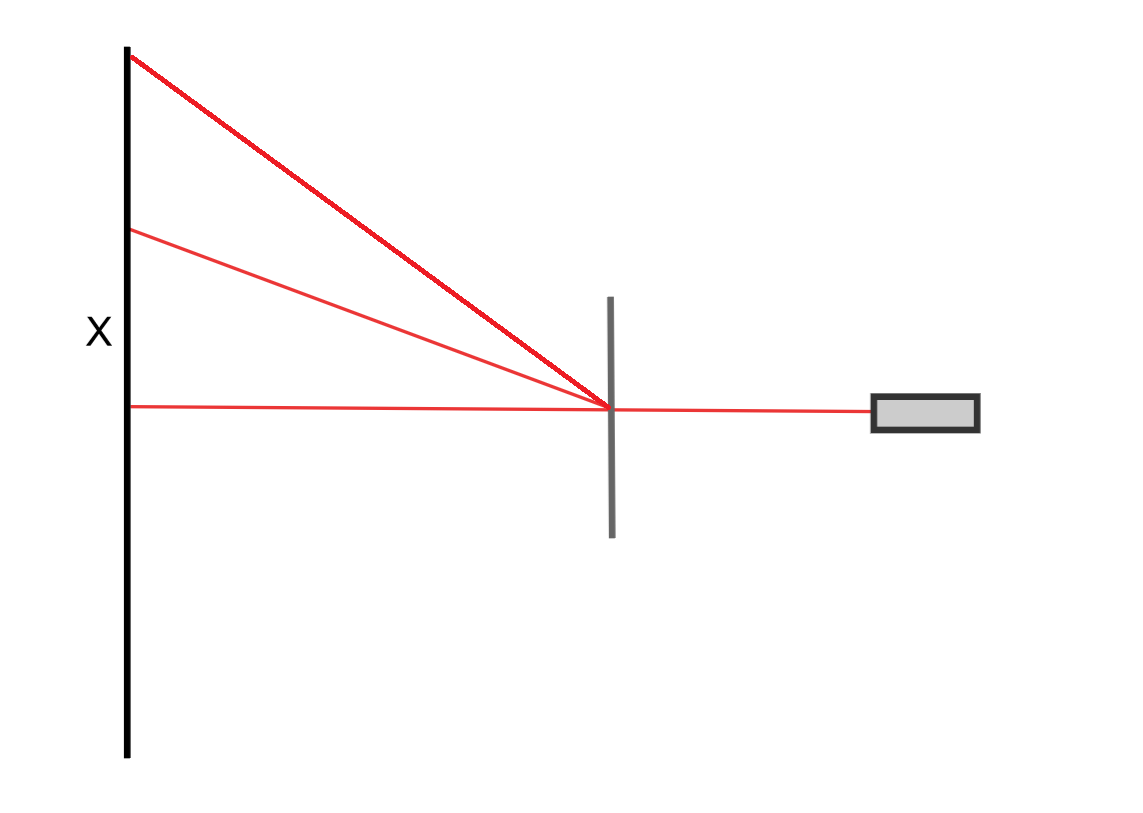
\includegraphics[scale=0.5]{skica.png}
\end{center}
\section*{Meritve:}

Označimo kot $d$ razdaljo med mrežico in zaslonom. Označimo kot $x_1$ razdaljo med 0. ojačitev in 1. ojačitev. Označimo kot $x_2$ razdaljo med 0. ojačitev in 2. ojačitev. 
Potem so izmerjeni podatki sledeči:


\begin{table}[H]
   \centering
\begin{tabular}{ll}
   $x_1$ & 0.60m \\
   $x_2$ & 1.485m \\
   $d$ & 1.77m \\
   $a$ & $\frac{1}{600}[mm]$
\end{tabular}
\end{table}


\section*{Rezultati in obdelava podatkov:}

\begin{multicols}{2}
Za interferenco velja naslednja enačba:
\begin{equation}
   a\sin{\phi} = N\lambda
\end{equation}

\columnbreak

$\tan{\phi}$ je enak:
\begin{equation}
   \tan{\phi} = \frac{x}{d}
\end{equation}

\end{multicols}

Lahko dokažemo da je:
\begin{equation}
   \sin{\phi} = \sqrt{\frac{\tan{\phi}^2}{1+ \tan{\phi}^2}}
\end{equation}
Kar pomeni da je:
\begin{equation}
   \sin{\phi} = \sqrt{\frac{x^2}{d^2 + x^2}}
\end{equation}
Posledično:
\begin{equation}
   a\sqrt{\frac{x^2}{d^2 + x^2}} = N\lambda
\end{equation}
Iz tega sledijo rezultati:
\begin{table}[H]
   \centering
\begin{tabular}{ll}
   & $\lambda[nm]$  \\
1 & 535\\
2 & 536\\
\end{tabular}
\end{table}

 

\section*{Dodatek}
Namesto izvora enobarvne svetlobe uporabi svetilko z belo svetlobo. Postavi režo in uklonsko mrežico tako, da na zaslonu dobiš spekter. Določi valovno dolžino rdeče, zelene in vijolične svetlobe.
\subsection*{Skica:}
\begin{center}
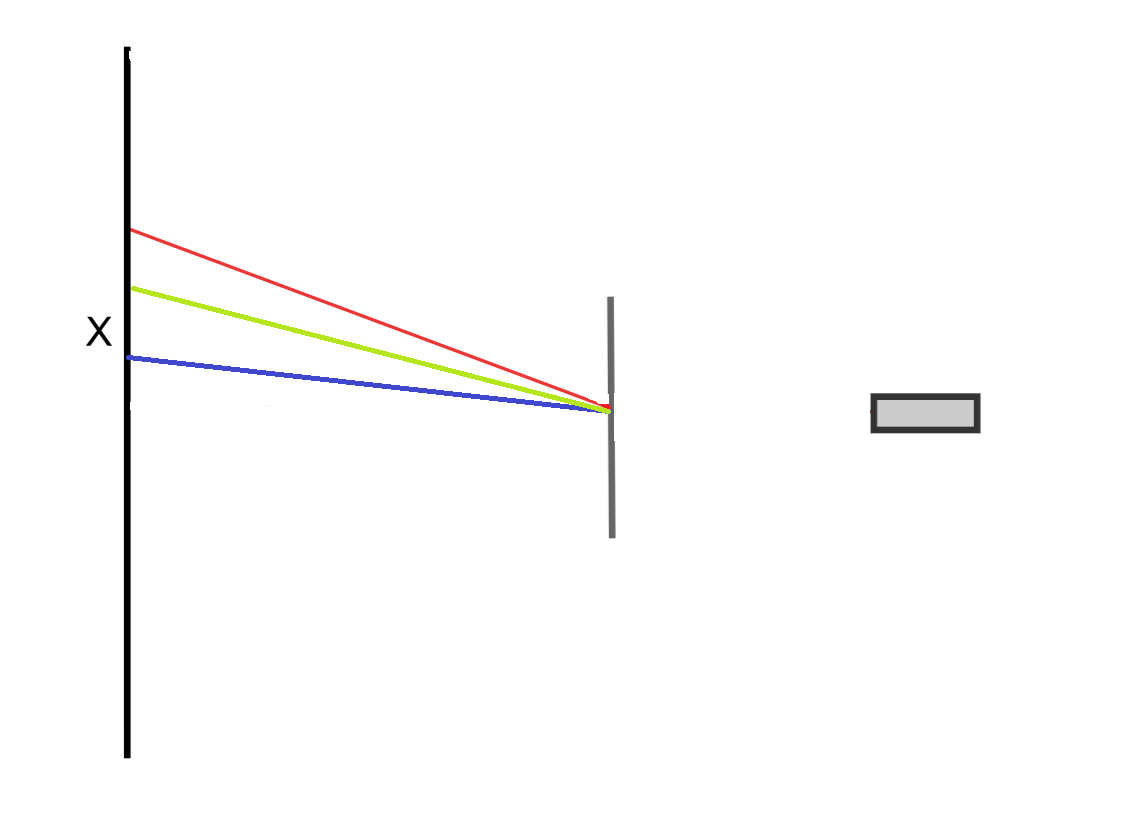
\includegraphics[scale=0.5]{skica2.png}
\end{center}
\subsection*{Meritve:}
\begin{table}[H]
   \centering
\begin{tabular}{ll}
   & $d[cm]$  \\
vijolična & 8\\
zelena & 10\\
rdeča & 12\\
\end{tabular}
\end{table}
\subsection*{Obdelava podatkov:}
Poleg zgoraj navedenih, so definirani še podatki:
\begin{gather}
   a = \frac{1}{100}[mm] \\
   d = 177cm \\
   N = 1 \\
\end{gather}
Iz tega potem lahko uporabimo enačbo:
\begin{equation}
   a\sqrt{\frac{x^2}{d^2 + x^2}} = N\lambda
\end{equation}
Kjer dobimo rezultate:
\begin{table}[H]
   \centering
\begin{tabular}{ll}
   & $\lambda[nm]$  \\
vijolična & 450\\
zelena & 560\\
rdeča & 680\\
\end{tabular}
\end{table}
\section*{Interpretacija:}

Razlogi za napake so povezani z nenatančnimi podatki o uklonski mrežici, ne popolnoma vzporedna postavitev zaslona na mrežico in napake v merjenju razdalj. 
\end{document}